\documentclass{article}
\usepackage[a4paper,top=2cm,bottom=2cm,left=2cm,right=2cm]{geometry}
\usepackage[english]{babel}
\usepackage[utf8]{inputenc}
\usepackage{fancyhdr}
\usepackage{float}
\usepackage{graphicx}
\usepackage{wrapfig}
\usepackage{siunitx} %per scrivere il simbolo °
\usepackage{verbatim} %per i commenti1
\usepackage{subfig}
\usepackage{amsmath}
\usepackage{algorithm}
\usepackage{algpseudocode}
\setcounter{secnumdepth}{3}
\setcounter{tocdepth}{6}
\usepackage{multirow}
\newcommand{\minitab}[2][l]{\begin{tabular}#1 #2\end{tabular}}
\usepackage{rotating}
\usepackage{xfrac}
\usepackage{cite}

\DeclareMathOperator*{\argmax}{arg\,max}
\DeclareMathOperator*{\argmin}{arg\,min}

%\usepackage{booktabs,array}
%\usepackage{tikz}

%\usepackage{tabularx}

%\usepackage{chngcntr}
%\counterwithin{table}{section}

%------------------------------ colors
\usepackage[usenames,dvipsnames,table]{xcolor} % use colors on table and more
\definecolor{333}{RGB}{51, 51, 51} % define custom color
\definecolor{background}{RGB}{248, 248, 255}
\definecolor{comment}{RGB}{17,167,5}
\definecolor{keyword}{RGB}{195,47,8}
\definecolor{string}{RGB}{142,195,0}
\definecolor{number}{RGB}{90,84,84}
\definecolor{identifier}{RGB}{0,90,201}

%------------------------------ source code
\usepackage{listings}

\lstset{
  basicstyle=\footnotesize\sffamily,
  commentstyle=\itshape\color{gray},
  captionpos=b,
  frame=shadowbox,
  language=HTML,
  rulesepcolor=\color{333},
  tabsize=2
}

\lstdefinestyle{code}{
  backgroundcolor=\color{background},
  basicstyle=\footnotesize\sffamily,
  commentstyle=\color{comment},
  frame=L,
  identifierstyle=\color{identifier},
  keywordstyle=\color{keyword},
  numbers=left,
  numbersep=10pt,
  numberstyle=\tiny\color{number},
  stringstyle=\color{string},
  showstringspaces=false,  
  stepnumber=1,
  tabsize=2
}

\title{\textbf{Report about Lab4}} % Title
\author{Raffaele \textsc{Di Nardo Di Maio} 1204879} % Author name
\date{\today}

\begin{document}
\begin{minipage}{.20\textwidth}
  
\includegraphics[height=3cm]{../Icon4}
\end{minipage}\begin{minipage}{.20\textwidth}
  \begin{table}[H]
  \begin{tabular}{l}
  \scshape{\Large{Computer Engineering Master Degree}} \\
  \hline \\
  \scshape{\Large{Computer Vision}} \\
  \end{tabular}
  \end{table}
\end{minipage}
{\let\newpage\relax\maketitle}

\section{Goal of the experience}
The goal of this lab experience was to detect street and a street signal in an image, highlighting them respectively with red and green colors. The extraction of them was done by using Canny edge detector and Hough transforms and tuning their parameters.
\section{Organization of code}
The code of this lab is organized in ten main files:
\begin{itemize}
\item{\textbf{Lab4.cpp} and its header file \textbf{Lab4.h}\\
they are associated to the \textit{main()} in which an instance of \textit{StreetDetector()} is created and its function \textbf{detect()} is called;}
\item{\textbf{StreetDetector.cpp} and its header file \textbf{StreetDetector.h}\\
these are used to create the class \textit{StreetDetector}, which its main function called \textbf{detect()}, that creates all the windows for Canny detector and Hough transforms, creating objects of the classes that implement them. In this function, the main flow of the program is managed and this is organized in two main phases:
\begin{enumerate}
\item{\textbf{Detection of street}\\
on screen there are two windows in the same time (Canny edge detection and Hough lines transform windows) and updating the first one, the second one is affected also by these changes. When one key, between 'q','ESC' and '\textbackslash{r}', is pressed by user, the last image in the Hough line window is used for the next part;
}
\item{\textbf{Detection of signal}\\
Using previously computed image, a new window is created for Hough Circle Transform;
}
\end{enumerate}
}
\item{\textbf{CannyDetector.cpp} and its header file \textbf{CannyDetector.h}\\
these are used to create the class \textit{CannyDetector};, that performs Canny edge detection}
\item{\textbf{HoughLinesDetector.cpp} and its header file \textbf{HoughLinesDetector.h}\\
these are used to create the class \textit{HoughLinesDetector};, that performs Hough transform detection for lines and highlights in red the triangle in the image, obtained by two most significant detected lines if they intersect;}
\item{\textbf{HoughCirclesDetector.cpp} and its header file \textbf{HoughCirclesDetector.h}\\
these are used to create the class \textit{HoughCirclesDetector};, that performs Hough transform detection for circles and highlights in green the most significant circle in the image, between all detected circles;}
\end{itemize}
\section{Command line parameters}
The program needs to have, as command line argument, the specification of the path of the image, including also the name of the image, on which you want to detect street and signal. 
\section{Experimental results}
In the following part there are the resulting images used in my workflow, to detect the circle and the image:\\
\begin{enumerate}
\item{\textbf{Evaluation of parameters of Canny detection and Hough lines transform}\\
Before applying the Canny Detection, to reduce hysteresis thresholds values, I apply a Blur filter of size 9x9. After this smoothing step, I apply Canny Detector and after Hough Lines transform. The most significant parameters of these detectors are respectively the first threshold and the angle resolution.
}
\item{\textbf{Evaluation of parameters of Hogh circles transform}\\
The most significant parameters of Hough Circles transform are max radius, if fixed min radius to 1, and the second method parameter. By changing second method parameter, the range of maximum radius, that highlights the signal, changes.  
}
\end{enumerate}
In Table \ref{param}, there are the parameters I used to obtain good detection of street and signal. In Figure \ref{result}, there is the image obtained by the program, using specified parameters at construction of objects, with detected street and signal. 
\begin{table}[h]
\centering
\begin{tabular}{|c|l|c|}
\hline
\multirow{2}{*}{Canny Detector}&{$threshold_1$}&{$[0.0, 157.0]$}\\
\cline{2-3}
&{$threshold_2$}&{$200$}\\
\hline
\multirow{3}{*}{Hough Lines Detector}&{\textit{distance resolution}}&{$1$}\\
\cline{2-3}
&{\textit{angle resolution}}&{$\frac{37\cdot \pi}{150}$}\\
\cline{2-3}
&{accumulator threshold}&{[0,14]}\\
\hline
\multirow{3}{*}{Hough Circles Detector}&{\textit{minimum distance}}&{$69.0$}\\
\cline{2-3}
&{\textit{parameter 1}}&{$30.0$}\\
\cline{2-3}
&{\textit{parameter 2}}&{$23.0$}\\
\cline{2-3}
&{\textit{minimum radius}}&{$1$}\\
\cline{2-3}
&{\textit{maximum radius}}&{$[10-21]$}\\
\hline
\end{tabular}
\caption{Estimated parameters of detectors that highlights signal and street.}\label{param}
\end{table}
\begin{figure}[h]
\begin{center}
  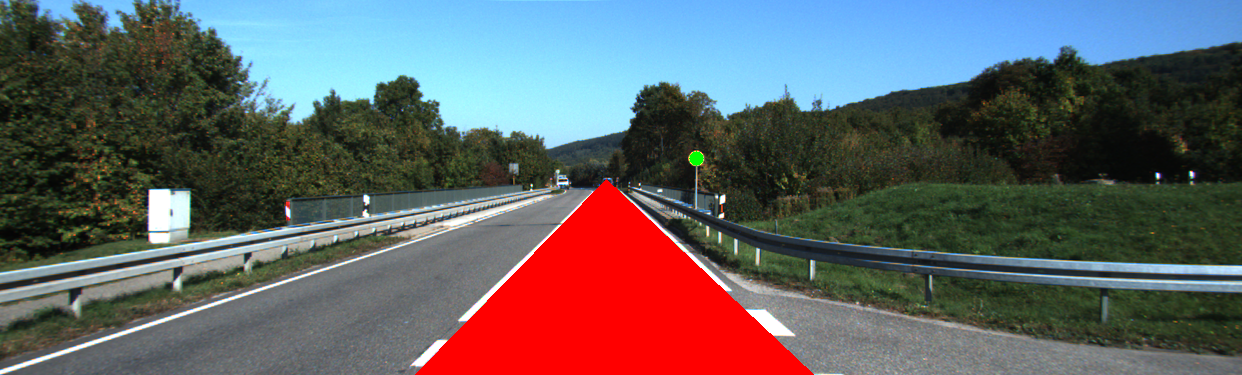
\includegraphics[scale=0.38]{result}\\ 
  \caption{\footnotesize{Image with highlighted street in red and signal in green.}}\label{result} 
\end{center} 
\end{figure}

\end{document}
